
\documentclass[twoside,12pt]{article}

\usepackage{dsctemplate}
\usepackage[margin=1in]{geometry}
\usepackage{amsmath}
\usepackage{amssymb,amsthm}
\usepackage{fancyhdr}
\usepackage{nicefrac}
\usepackage{minted}
\usetikzlibrary{quotes,angles,positioning,arrows.meta}
\usetikzlibrary{calc}
\usepackage{enumitem}
\usepackage{fancyvrb}
\usepackage{dirtytalk}
\usepackage{comment}
\usepackage{minted}
\usepackage{subfigure}
\usepackage{subcaption}

\DefineVerbatimEnvironment{verbatim}{Verbatim}{xleftmargin=.5in}
\newlist{multiplechoice}{itemize}{2}
\setlist[multiplechoice]{label=$\square$}

% configuration
% ------------------------------------------------------------------------------

% control whether solutions are shown or hidden
% \showsolntrue

% page headers only on odd pages
\pagestyle{fancy}
\fancyhead{}
\fancyhead[RO]{uniqname: \rule{3in}{.5pt}}
\renewcommand{\headrulewidth}{0pt}
% \pagenumbering{gobble}

% ------------------------------------------------------------------------------

\begin{document}


\thispagestyle{empty}

\vspace{-5.5in}

\pstitle{%
    Midterm Exam
}{EECS 398, Winter 2025}

\vspace{-.3in}

\begin{tabular}{rl}
    Full Name: & \inlineresponsebox[4in]{Solutions}\\
    Uniqname: & \inlineresponsebox[4in]{rampure}\\
    UMID: & \inlineresponsebox[4in]{12345678} \vspace{0.2in} \\
    Room: & \begin{tabular}{lll}\bubble{1010 DOW} & \bubble{1013 DOW} & \bubble{1017 DOW} \\ 
    \bubble{1018 DOW} & \bubble{2311 EECS} & \bubble{TAC} \end{tabular}\vspace{.1in} \\ 
\end{tabular}

\vspace{.1in}

\hline

\vspace{.1in}


\textbf{Instructions:}
    \begin{itemize}
        \item You have 120 minutes to complete this exam.
        \item This exam consists of 15 questions, worth a total of 90 points.
        \item Write your uniqname in the top right corner of each page in the space provided.
        \item Please write \textbf{clearly} in the provided answer boxes; we will not grade work that appears elsewhere. Completely fill in bubbles and square boxes; if we cannot tell which option(s) you selected, you may lose points.
        
            \bubble{A bubble means that you should only \textbf{select one choice}.}
            
            \squarebubble{A square box means you should \textbf{select all that apply}.}
            
        \item You may refer to a single two-sided handwritten notes sheet. Other than that, you may not refer to any other resources or technology during the exam (no phones, watches, or calculators).
    \end{itemize}

\vspace{.1in}

\hline

\vspace{0.1in}

\noindent You are to abide by the University of Michigan/Engineering Honor Code. To receive a grade,
please sign below to signify that you have kept the honor code pledge.

\vspace{0.2in}

\noindent \textit{I have neither given nor received aid on this exam, nor have I concealed any violations of the
Honor Code.}

\vspace{0.2in}

\begin{tabular}{rl}
    \: \: \: \: \: Signature: & \biginlineresponsebox[4in]{}\\
\end{tabular}

\begin{center}

\vspace{0.3in}

% \huge{Version A}

\end{center}

\newpage

\begin{center}
    \noindent \textbf{\large{Data Overview: Food Deliveries}} 
\end{center}

\noindent In this exam, we'll work with the DataFrame \texttt{orders}, which contains information about deliveries made using various food delivery services in India.

\vspace{.1in}

\noindent The first few rows of \texttt{orders} are shown below, but \texttt{orders} has many more rows than are shown.

% \vspace{-.5in}

\begin{center}

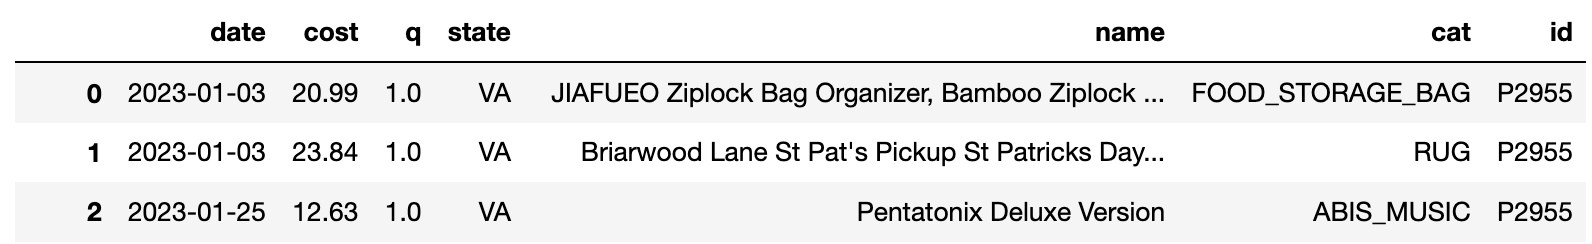
\includegraphics[width=0.7\textwidth]{midterm-images/df.png}

\end{center}

\vspace{.1in}

\noindent Each row in \texttt{orders} contains information about a single delivery. The columns in \texttt{orders} are as follows:

\begin{itemize}

\item \texttt{"driver" (str)}: The delivery driver's ID. Note that there are duplicate values in this column, because some drivers have made multiple deliveries.
\item \texttt{"type" (str)}: The type of food ordered; either \texttt{"Buffet"}, \texttt{"Drinks"}, \texttt{"Meal"}, or \texttt{"Snack"}.
\item \texttt{"rating" (float)}: The average rating of the driver out of 5, \textbf{after} making the given delivery.
\item \texttt{"dist" (float)}: The distance from the restaurant to the delivery address, in kilometers.
\item \texttt{"traffic" (str)}: The level of traffic; either \texttt{"High"}, \texttt{"Low"}, \texttt{"Moderate"}, or \texttt{"Very High"}.
\item \texttt{"minutes" (float)}: The time in minutes between when a customer places their order and when they receive it.

\end{itemize}

\noindent \textbf{Throughout the exam}, assume we have already run all necessary import statements.

\newpage

\noindent \textbf{Make sure you have read the Data Overview before beginning!}

\begin{probset}

\begin{prob}[(4 pts)]

Driver \texttt{"WOLVAA01"} has made several deliveries. Write an expression that evaluates to the number of minutes \texttt{"WOLVAA01"} took to deliver their \textbf{second}-fastest order.

\begin{responsebox}{1.25in}

\end{responsebox}

\end{prob}

\vspace{0.2in}

\begin{prob}[(5 pts)]

Drivers' ratings can change over time, as they perform more and more deliveries. For instance, after one delivery a driver's rating might be 4.8, and after their next delivery it might drop to 4.7. We say a driver is \textit{consistent} if their rating was the \textbf{exact same} for all of their deliveries in \texttt{orders}.

Fill in the blanks so \texttt{prop\_consistent} below evaluates to a float, corresponding to the \textbf{proportion of drivers} who are consistent.

\begin{verbatim}
def f(x):
    return __(iv)__

prop_consistent = (
 orders
 .groupby(__(i)__)
 [__(ii)__]
 .__(iii)__(f)
 .mean()
)
\end{verbatim}

\begin{tabular}{ll}

\texttt{(i)}: & \inlineresponsebox[2.5in]{} \hspace{0.35in} \texttt{(ii)}: \inlineresponsebox[2.5in]{} \\ \\ 
\texttt{(iii)}: & \bubble{\texttt{agg}} \bubble{\texttt{filter}} \bubble{\texttt{transform}} \\ \\ 
\texttt{(iv)}: & \biginlineresponsebox[6in]{}

\end{tabular}

\end{prob}

\newpage

\begin{prob}[(3 pts)]

Suppose the expression below evaluates to \texttt{1}.

\begin{verbatim}
(orders[orders["type"] == "Snack"]["driver"]
 .value_counts()
 .value_counts()
 .shape[0]
)
\end{verbatim}

What can we conclude about \texttt{orders}?

\begin{tabular}{l}
\bubble{Every driver made at least 1 \texttt{"Snack"} delivery.} \\

\bubble{Every driver made exactly 1 \texttt{"Snack"} delivery.} \\

\bubble{Every driver made at most 1 \texttt{"Snack"} delivery.} \\

\bubble{Every driver made exactly $k$ \texttt{"Snack"} deliveries, where $k$ is some positive constant.} \\

\bubble{Every driver made exactly 0 or exactly $k$ \texttt{"Snack"} deliveries, where $k$ is some positive constant.} \\

\bubble{Every driver that made a \texttt{"Snack"} delivery did not make any other kind of delivery.}

\end{tabular}

\end{prob}

\vspace{0.2in}

\begin{prob}[(3 pts)]

In one English sentence, describe what the following expression computes. Your sentence should start with ``The driver", and should be understandable by someone who has never written code before, i.e. it should not use any technical terms. 

\begin{verbatim}
(orders
 .groupby("driver")
 .filter(lambda df: df.shape[0] >= 10 and df["rating"].min() >= 4.5)
 .groupby("driver")
 ["minutes"]
 .sum()
 .idxmax()
)
\end{verbatim}

\begin{responsebox}{2in}
    
\end{responsebox}

\end{prob}

\newpage

\begin{prob}[(6 pts)]

Consider the DataFrame \texttt{C}, defined below.

\begin{verbatim}
C = orders.pivot_table(
  index="type", # Possible values: "Buffet", "Drinks", "Meal", "Snacks"
  columns="traffic", # Possible values: "High", "Low", "Moderate", "Very Low"
  values="minutes",
  aggfunc="count"
)
\end{verbatim}

Throughout this question, assume that after defining \texttt{C} above, \textbf{we sort \texttt{C} such that both its index and columns are in ascending alphabetical order} (as shown above).

\begin{subprobset}

\begin{subprob}(3 pts) Fill in the blanks so that the expression below evaluates to the \textbf{proportion of \texttt{"Snack"} deliveries that were made in \texttt{"Moderate"} traffic}. Each blank should be filled with a single integer, float, string, or Boolean value.

\begin{verbatim}
C.iloc[__(i)__, __(ii)__] / C.loc[__(iii)__].sum()
\end{verbatim}

\texttt{(i)}: \inlineresponsebox[1.5in]{} \texttt{(ii)}: \inlineresponsebox[1.5in]{} \texttt{(iii)}: \inlineresponsebox[1.5in]{}

\end{subprob}

\vspace{0.2in}

\begin{subprob}(3 pts) Fill in the blanks so that the expression below evaluates to the \textbf{proportion of deliveries made in \texttt{"Low"} traffic that were for \texttt{"Buffet"}s}. Blanks (i) and (ii) should each be filled with a single integer, float, string, or Boolean value.

\begin{verbatim}
C.loc[__(i)__, __(ii)__] / __(iii)__.sum()
\end{verbatim}

\texttt{(i)}: \inlineresponsebox[1.5in]{} \texttt{(ii)}: \inlineresponsebox[1.5in]{} 

\texttt{(iii)}: 
\begin{tabular}{lll}
\bubble{\texttt{C.iloc[:, -1]}} & \bubble{\texttt{C.iloc[:, 0]}} & \bubble{\texttt{C.iloc[:, 1]}} \\
\bubble{\texttt{C.iloc[-1, :]}} & \bubble{\texttt{C.iloc[0, :]}} & \bubble{\texttt{C.iloc[1, :]}}
\end{tabular}

\end{subprob}

% \begin{subprob}(2 pts) In one English sentence, describe what the following expression computes. Your sentence should be understandable by someone who has never written code before, i.e. it should not use any technical terms. 

% \begin{verbatim}
% C.idxmax(axis=1)
% \end{verbatim}

% \begin{responsebox}{1.25in}
    
% \end{responsebox}

% \end{subprob}

\end{subprobset}

\end{prob}

\newpage

\begin{prob}[(9 pts)]

Consider the DataFrames \texttt{A} and \texttt{B}, shown below in their entirety.

\begin{center}

    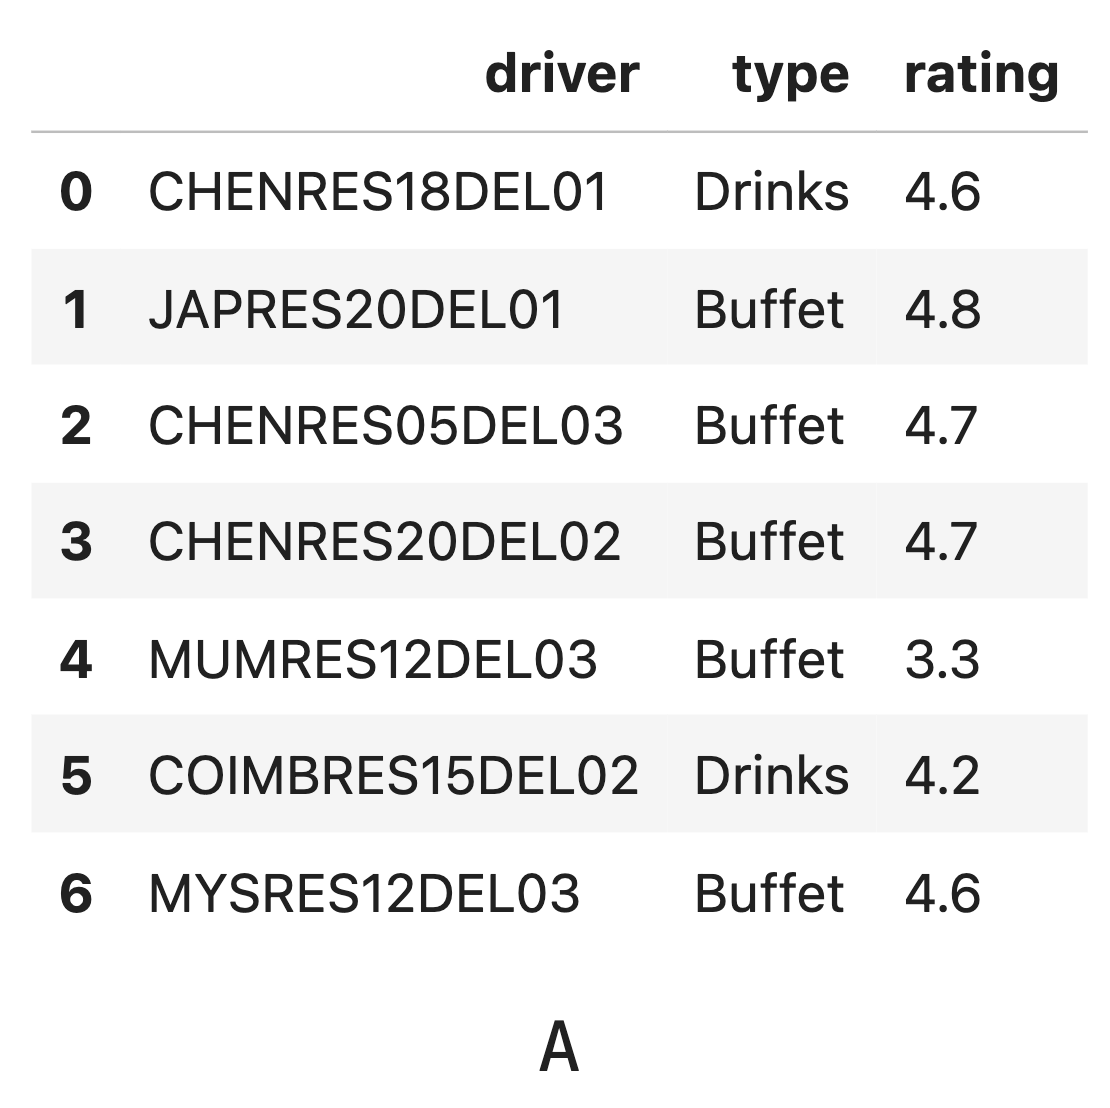
\includegraphics[width=0.4\textwidth]{midterm-images/A.png}
    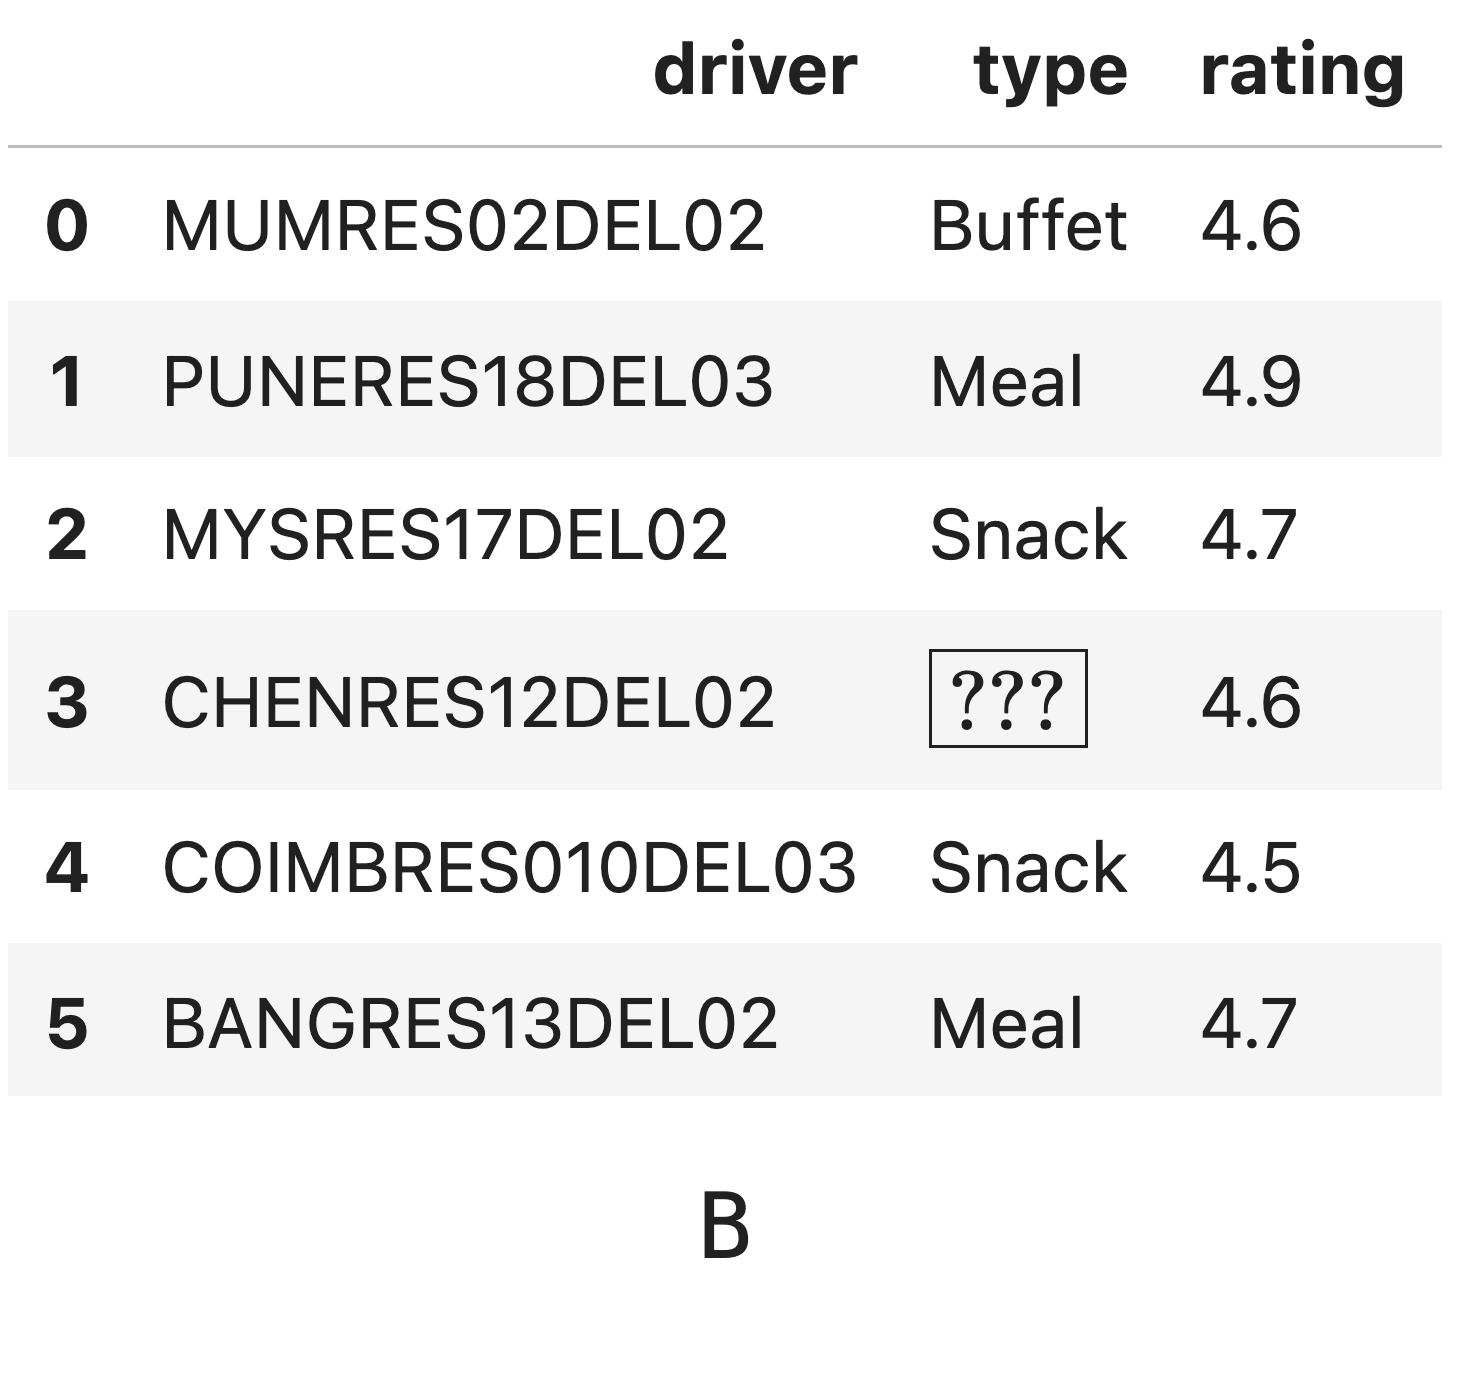
\includegraphics[width=0.4\textwidth]{midterm-images/B.png}

\end{center}

\vspace{-0.2in}

Note that the \texttt{"type"} value in row \textbf{3} of DataFrame \texttt{B} is unknown. Remember from the Data Overview page that the only possible values in the \texttt{"type"} column are \texttt{"Buffet"}, \texttt{"Drinks"}, \texttt{"Meal"}, and \texttt{"Snack"}.

\begin{subprobset}

\begin{subprob}(2 pts) Suppose the DataFrame \texttt{A.merge(B, on="type")} has \texttt{7} rows.

What must the unknown value, $\boxed{\text{???}}$, be?
   \bubble{Drinks} 
   \bubble{Buffet} 
   \bubble{Meal} 
   \bubble{Snack}

\end{subprob}

\vspace{0.3in}

\begin{subprob}(2 pts) Suppose the DataFrame \texttt{A.merge(B, on="type")} has \texttt{10} rows.

What must the unknown value, $\boxed{\text{???}}$, be?

  \bubble{\texttt{"Drinks"}} 
  \bubble{\texttt{"Buffet"}} 
  \bubble{\texttt{"Meal"}} 
  \bubble{\texttt{"Snack"}}  

\end{subprob}

\vspace{0.3in}

\begin{subprob}(3 pts) Suppose the DataFrame \texttt{A.merge(B, on="type", how="outer")} has $k$ rows. The value of $k$ depends on the unknown value, $\boxed{\text{???}}$.

Which integer below \textbf{cannot} be $k$?

% Three of the following four options \textit{could} be the value of $k$. Which option \textbf{cannot} be the value of $k$?

% Which of the following numbers \textbf{cannot be} the number of rows in the DataFrame ?

\bubble{11} 
\bubble{12} 
\bubble{14} 
\bubble{16}

% \begin{responsebox}{1.5in}
    
% \end{responsebox}

\end{subprob}

\vspace{0.9in}

\begin{subprob}(2 pts) Suppose the unknown value, $\boxed{\text{???}}$, is \texttt{"Buffet"}.

How many rows are in the DataFrame \texttt{A.merge(B, on=["type", "rating"])}?

\bubble{0} 
\bubble{1} 
\bubble{2} 
\bubble{3} 
\bubble{4} 
\bubble{5} 
\bubble{6} 
\bubble{7}

\end{subprob}

\end{subprobset}

\end{prob}

\newpage

\begin{prob}[(7 pts)]

The delivery company wants to reward a subset of its drivers with a gift card for their service. To do so, they:

\begin{enumerate}
    \item Choose an integer $k$ between 1 and 10 inclusive, uniformly at random.
    \item Choose $k$ \textbf{unique} drivers, uniformly at random, such that all drivers have the same chance of being chosen, no matter how many deliveries they have made. Note that a driver cannot be selected more than once.
\end{enumerate}

Driver \texttt{"WOLVAA01"} asks ChatGPT to write code that simulates the probability that he wins a gift card, and it gives him back the following:

\begin{verbatim}
drivers = orders["driver"].unique()

def choose_k():
    return np.random.choice(np.arange(1, 11))

def one_sim(k):
    selected = np.array([])
    for i in range(k):
        selectee = np.random.choice(drivers, 1, replace=False)
        selected = np.append(selected, selectee)
    return "WOLVAA01" in selected

def simulation():
    k = choose_k()
    N = 100_000
    total = 0
    for i in range(N):
        total = total + one_sim(k)
    return total / N
\end{verbatim}

\texttt{simulation()} \textit{should} return an estimate of the probability that \texttt{"WOLVAA01"} wins a gift card, but some of the code is potentially buggy. \textbf{Select all issues} with the code above.

% \squarebubble{When defining \texttt{drivers} in line \texttt{1}, we should use the \texttt{.unique()} method on \texttt{orders["driver"]}.}

\squarebubble{\texttt{drivers} only includes the drivers that made one delivery, rather than all drivers.}

\squarebubble{\texttt{choose\_k} returns a random integer between \texttt{1} and \texttt{11}, instead of one from \texttt{1} to \texttt{10}.}

\squarebubble{\texttt{choose\_k} always returns the same number.}

\squarebubble{\texttt{one\_sim} draws \texttt{k} drivers with replacement, instead of without replacement.}

\squarebubble{\texttt{one\_sim} draws \texttt{k} drivers without replacement, instead of with replacement.}

\squarebubble{\texttt{one\_sim} always returns \texttt{False}, because \texttt{selected} is always an empty array.}

\squarebubble{\texttt{simulation} only picks one value of \texttt{k}, when it should select a new \texttt{k} on each iteration.}

\squarebubble{None of the above.}

% \begin{subprobset}

% \begin{subprob}

% Where is the issue created?

% \bubble{The definition of \texttt{drivers} in line \texttt{1}}

% \bubble{The definition of \texttt{choose\_k} in line \texttt{2}}

% \bubble{The definition of \texttt{one\_sim} in lines \texttt{4-9}}

% \bubble{The definition of \texttt{simulation} in lines \texttt{11-17}}

% \end{subprob}

% \begin{subprob}

% What is the issue?

% \begin{responsebox}{1in}
    
% \end{responsebox}

% \end{subprob}

% \end{subprobset}


% Which of the following are flawed?

% Below, state all issues with the code above, and how you would fix them. Your answer should refer to specific line numbers.

% \begin{responsebox}{2.25in}
    
% \end{responsebox}

\end{prob}

\newpage

\begin{prob}[(9 pts)]

Suppose the DataFrame \texttt{D} contains a subset of the rows in \texttt{orders}, such that:

\begin{itemize}
    \item Some of the values in the \texttt{"minutes"} column are missing.
    \item None of the values in the \texttt{"minutes"} column are missing for orders made in \texttt{"Moderate"} traffic.
\end{itemize}

% Consider the DataFrame \texttt{D}, shown below \textbf{in its entirety}.

% \vspace{-0.1in}

% \begin{center}

% 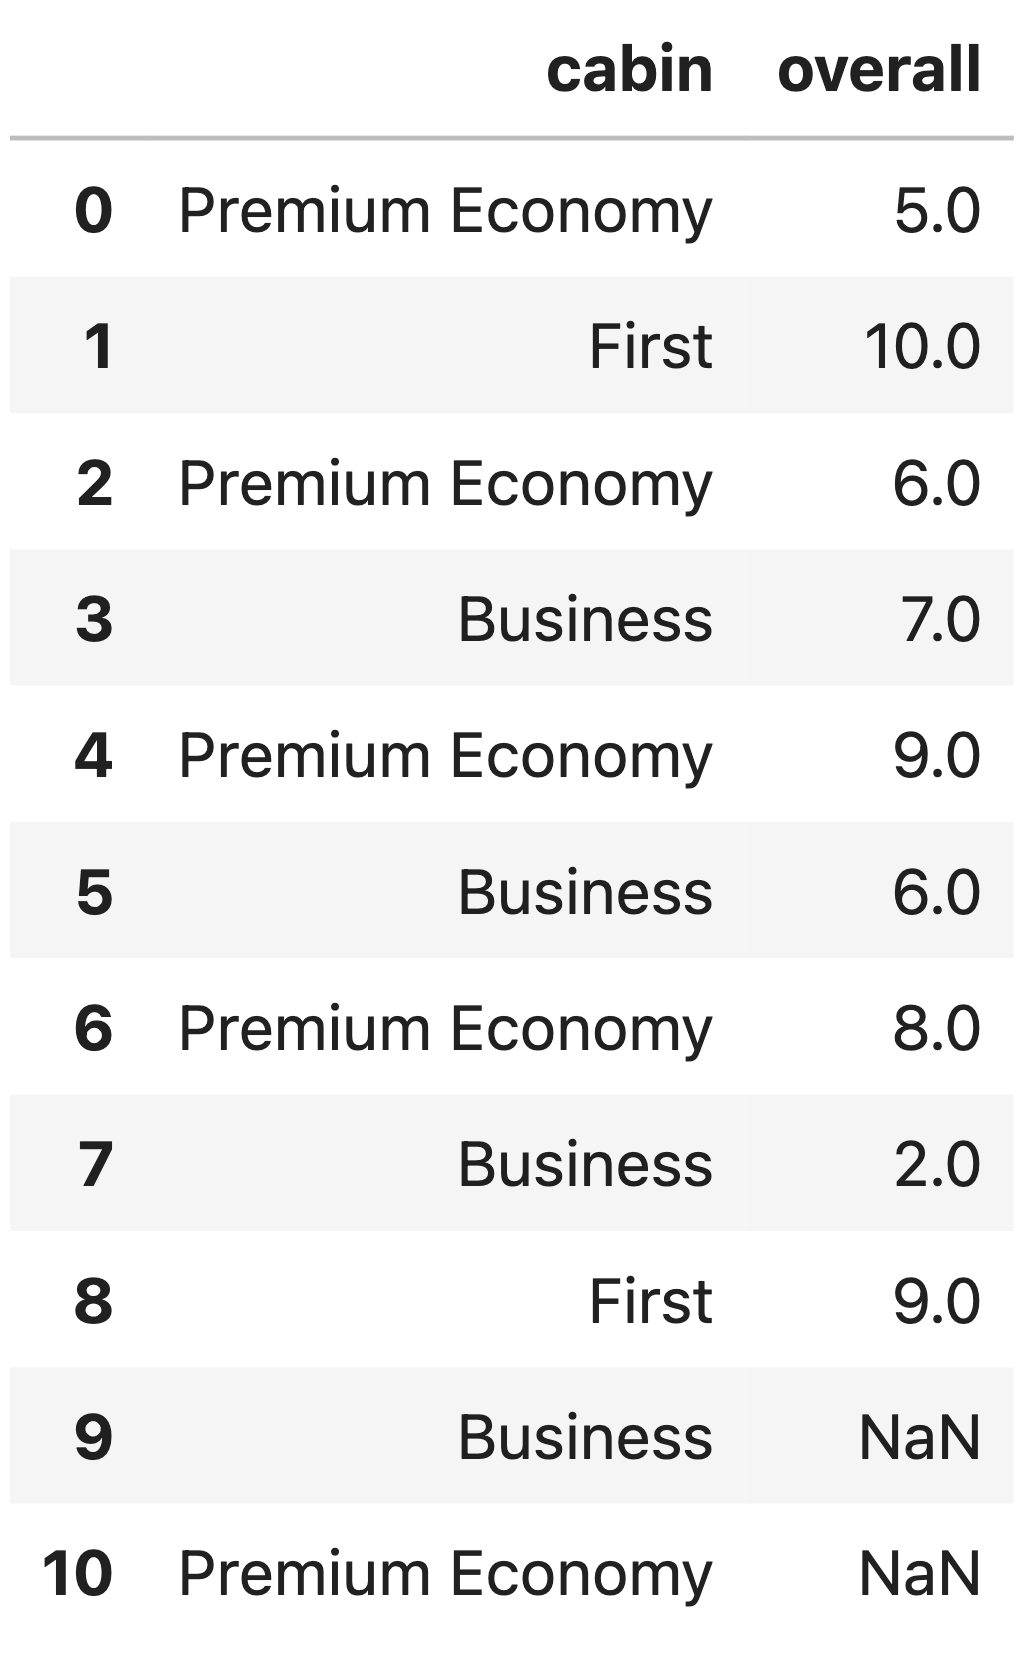
\includegraphics[width=0.25\textwidth]{midterm-images/imp.png}

% \end{center}

% \vspace{-0.15in}

Each part of this question is independent of all other parts. In each part, \textbf{select all} expressions that are \textbf{guaranteed} to evaluate to the \textbf{same} value, \textbf{before and after} the imputation code is run. The first part is done for you.

\begin{subprobset}

\begin{subprob}

\begin{verbatim}
t = lambda x: x.fillna(x.mean())
D["minutes"] = t(D["minutes"])
\end{verbatim}

\squarebubble{\texttt{D["minutes"].isna().sum()}}

\squarebubble[fill=black!90]{\texttt{D.shape[0] \# Correct; D.shape[0] doesn't change after the code above runs.}}

\end{subprob}

\end{subprobset}

% An explanation of part (a):

% \begin{itemize}
%     \item Before the two lines of code are run, \texttt{D["minutes"].isna().sum()} is some non-zero value (since some \texttt{"minutes"} values are missing), and after the two lines of code are run, \texttt{D["minutes"].isna().sum()} is \texttt{0}. 
    
%     Because \texttt{D["minutes"].isna().sum()} does not evaluate to the same value before and after, we did not select it.
%     \item Before the two lines of code are run, \texttt{D.shape[0]} is equal to the number of rows in \texttt{D}, which is not changing; since \texttt{D.shape[0]} does evaluate to the same value before and after, we selected it.
% \end{itemize}

% \newpage

% For your convenience, we show the DataFrame \texttt{D} again below in its entirety.

% \begin{center}

% 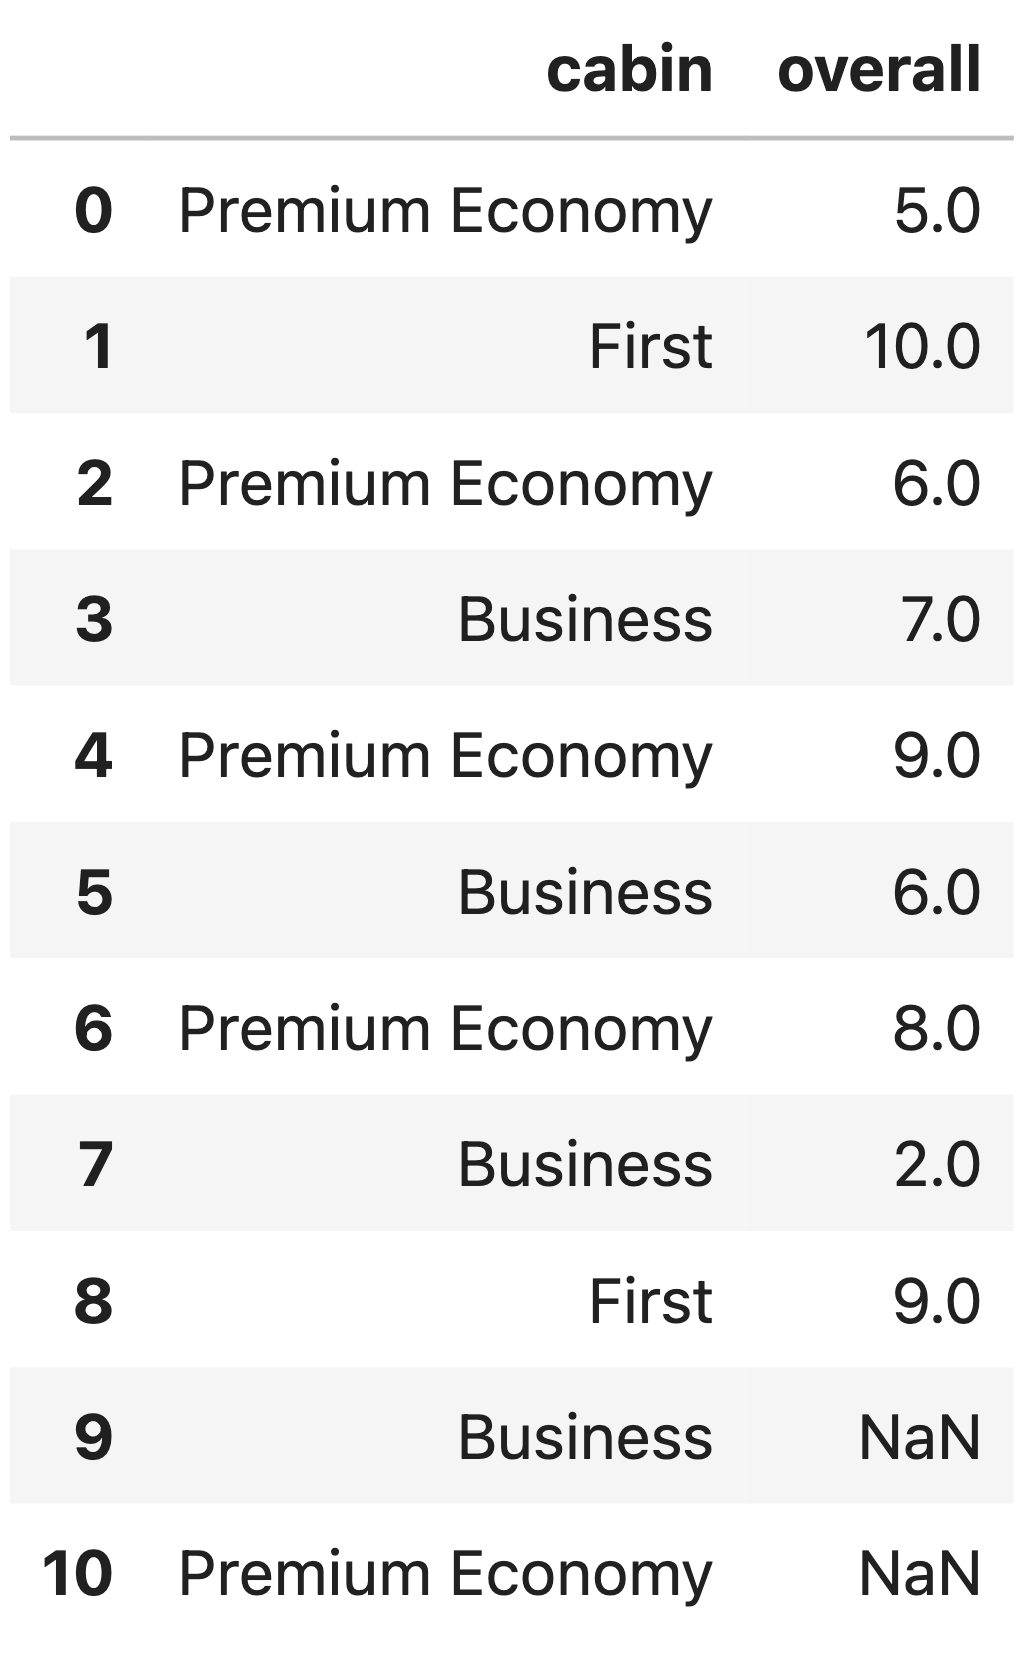
\includegraphics[width=0.25\textwidth]{midterm-images/imp.png}

% \end{center}

\begin{subprobset}

\begin{subprob}(3 pts)

\begin{verbatim}
t = lambda x: x.fillna(x.mean())
D["minutes"] = t(D["minutes"])
\end{verbatim}

\squarebubble{\texttt{D["minutes"].mean()}}

\squarebubble{\texttt{D.loc[D["traffic"] == "Moderate", "minutes"].mean()}}

\squarebubble{\texttt{D.groupby("traffic")["minutes"].mean()}}

\squarebubble{None of the above.}

\end{subprob}

\vspace{0.2in}

\begin{subprob}(3 pts)

\begin{verbatim}
t = lambda x: x.fillna(x.mean())
D["minutes"] = D.groupby("traffic")["minutes"].transform(t)
\end{verbatim}

\squarebubble{\texttt{D["minutes"].mean()}}

\squarebubble{\texttt{D.loc[D["traffic"] == "Moderate", "minutes"].mean()}}

\squarebubble{\texttt{D.groupby("traffic")["minutes"].mean()}}

\squarebubble{None of the above.}

\end{subprob}

\vspace{0.2in}

\begin{subprob}(3 pts)

\begin{verbatim}
present = D.loc[D["minutes"].notna(), "minutes"]
n = D["minutes"].isna().sum()
D.loc[D["minutes"].isna(), "minutes"] = np.random.choice(present, n)
\end{verbatim}

\squarebubble{\texttt{D["minutes"].mean()}}

\squarebubble{\texttt{D.loc[D["traffic"] == "Moderate", "minutes"].mean()}}

\squarebubble{\texttt{D.groupby("traffic")["minutes"].mean()}}

\squarebubble{None of the above.}

\end{subprob}

\end{subprobset}

\end{prob}

\newpage

\begin{prob}[(4 pts)]

In the DataFrame \texttt{orders}, assume that:

\begin{itemize}
    \item The median delivery time in \texttt{"Low"} traffic was 22 minutes.
    \item The median delivery time in \texttt{"Moderate"} traffic was 31 minutes.
    \item The median delivery time in \texttt{"High"} traffic was 42 minutes.
    \item The median delivery time in \texttt{"Very High"} traffic was 60 minutes.
\end{itemize}

Draw the following visualization, given the information you have.

\begin{verbatim}
orders.plot(kind="box", x="traffic", y="minutes")
\end{verbatim}

While it's not possible to draw the visualization exactly, since you don't have all of the exact delivery times, it is possible to roughly sketch it, such that the information provided above is clearly visible. Some additional instructions:
\begin{itemize}
    \item For simplicity, assume that across \texttt{"traffic"} categories, the variation in delivery times is roughly the same.
    \item Make sure your axes are labeled correctly. \textit{(Hint: The $y$-axis should have numerical labels.)}
\end{itemize}

\begin{responsebox}{4in}
    
\end{responsebox}

\end{prob}

\newpage

% \begin{prob}

% Just in this question, suppose that some of the values in the \texttt{"minutes"}

% \end{prob}

\newpage

\begin{prob}[(10 pts)]

Consider the following corpus of two documents:

\begin{enumerate}
    \item butter chicken $\underbrace{\text{naan naan ... naan}}_{k \text{\: ``naan"s total}}$
    \item curry with naan
\end{enumerate}

The total number of occurrences of ``naan" in document 1 is $k$, so the total number of terms in document 1 is $k + 2$, where $k \geq 3$ is some positive integer. Note that the two documents above are the only two documents in the corpus, meaning that there are 5 unique terms total in the corpus.

\begin{subprobset}

\begin{subprob}(4 pts) Given that the cosine similarity between the bag-of-words vector representations of the two documents is $\displaystyle \frac{5}{9}$, what is the value of $k$?

\bubble{3}
\bubble{4}
\bubble{5}
\bubble{6}
\bubble{7}
\bubble{8}
\bubble{9}
\bubble{10}

% Show your work, and $\boxed{\text{box}}$ your final answer, which should be an integer.

% \begin{responsebox}{3in}

% \end{responsebox}

\end{subprob}

\vspace{0.3in}

\begin{subprob}(3 pts) In this part, assume we are using a base-2 logarithm.

\begin{enumerate}[label=(\roman*)]

\item Which term in \textbf{document 1} has the largest TF-IDF?

If there are ties, select them all.

\squarebubble{butter} \squarebubble{chicken} \squarebubble{naan} \squarebubble{curry} \squarebubble{with}

\vspace{0.02in}

\item Which term in \textbf{document 2} has the largest TF-IDF?

If there are ties, select them all.

\squarebubble{butter} \squarebubble{chicken} \squarebubble{naan} \squarebubble{curry} \squarebubble{with}

\end{enumerate}

\end{subprob}

\vspace{0.1in}

\begin{subprob}(3 pts) This part is independent of the previous parts.

In practice, you'll encounter lots of new metrics and formulas that you need to make sense of on the job. For instance, the \textbf{Wolverine Score (WS)}, defined below, is an alternative to the TF-IDF that also tries to quantify the importance of a term $t$ to a document $d$, given a corpus of documents $d_1, d_2, ..., d_n$.

\vspace{-0.1in}

$$\text{WS}(t, d) = \left( \frac{\text{total \# of terms in $d$}}{\text{\# of occurrences of $t$ in $d$}} \right) \cdot   \left( \frac{\sum_{i=1}^n \text{\# of occurrences of $t$ in $d_i$}}{\sum_{i=1}^n \text{total \# of terms in $d_i$}}\right)$$

Fill in the blank to complete the statement below.

``If \texttt{\_\_\_\_}, then term $t$ is more common in document $d$ than it is across the entire corpus, and so $t$ is likely an important term in $d$."

What goes in the blank?

\bubble{$\text{WS}(t, d) < 0$}

\bubble{$\text{WS}(t, d) > 0$}

\bubble{$\text{WS}(t, d) < 1$}

\bubble{$\text{WS}(t, d) > 1$}

\bubble{$\text{WS}(t, d) < \frac{1}{n}$, where $n$ is the number of documents in the corpus}

\bubble{$\text{WS}(t, d) > \frac{1}{n}$, where $n$ is the number of documents in the corpus}

\end{subprob}

\end{subprobset}

\end{prob}

\newpage

% \begin{prob}


% \end{prob}

% \begin{subprobset}

% \begin{subprob}

% Consider the corpus of two documents below.

% \begin{enumerate}
%     \item $d_1$: butter chicken $\text{naan naan naan}$
%     \item $d_2$: curry with naan
% \end{enumerate}

% What is the value of $\text{CTF}(\text{``naan"}, d_1)$? Give your answer as a \textbf{simplified fraction}.

% \biginlineresponsebox[2in]{}

% \end{subprob}

% \vspace{0.2in}

% \begin{subprob}

% \end{subprob}

% \end{subprobset}

\newpage

\begin{prob}[(9 pts)]

The HTML document below contains the items on Wolverine Flavors Express' menu. We've only shown three menu items, but there are many more, as indicated by the ellipses \texttt{...}

\begin{verbatim}
<html>
    <head>
        <title>Wolverine Flavors Express: A2's Favorite Indian Spot</title>
    </head>
    <body>
        <h1>Wolverine Flavors Express Menu</h1>
        <div class="meta">Last Updated February 25, 2025</div>
        <div class="menu-item" data-price="14.99" data-calories="650">
            <h2>Butter Chicken</h2>
            <p>Tender chicken in creamy tomato sauce - $14.99</p>
        </div>
        <div class="menu-item" data-price="12.99" data-calories="480">
            <h2>Chana Masala</h2>
            <p>Spiced chickpea curry - $12.99 ($11.99 on Tuesday)</p>
        </div>
        ...
        <div class="menu-item" data-price="21.99" data-calories="1050">
            <h2>Chicken 65 Biryani</h2>
            <p>Spicy chicken marinated with rice - $21.99 (special)</p>
        </div>
    </body>
</html>
\end{verbatim}

Suppose we define \texttt{soup} to be a BeautifulSoup object that is instantiated using the HTML document above. Fill in the blanks below so that \texttt{low\_cals} contains the names of the menu items with less than 500 calories.

\begin{verbatim}
low_cals = []
for x in __(i)__:
    if __(ii)__:
        low_cals.append(__(iii)__)
\end{verbatim}

\begin{tabular}{ll}

\texttt{(i)}: &\inlineresponsebox[6in]{} \\

\texttt{(ii)}: &\inlineresponsebox[6in]{} \\

\texttt{(iii)}: &\inlineresponsebox[6in]{}

\end{tabular}

\end{prob}

\newpage

\begin{prob}[(6 pts)]

When we originally downloaded the \texttt{orders} dataset from the internet, some of the values in the \texttt{"minutes"} columns were formatted incorrectly as strings with two decimals in them. To clean the data, we implemented the function \texttt{clean\_minutes}, which takes in an invalid minutes value as a string and returns a correctly formatted minutes value as a float. Example behavior of \texttt{clean\_minutes} is given below.

% \vspace{-0.125in}

\begin{verbatim}
>>> clean_minutes("8.334.108")
83.34
>>> clean_minutes("5.123.999")
51.23
>>> clean_minutes("12.091.552")
120.91
>>> clean_minutes("525.345.262")
5253.45
\end{verbatim}

% \vspace{-0.125in}

As a helper function, we implemented the function \texttt{split\_pieces}; example behavior is given below.

\vspace{-0.125in}

\begin{verbatim}
>>> split_pieces("8.334.108")
("8", "334")
>>> split_pieces("12.091.552")
("12", "091")
\end{verbatim}

Fill in the blanks to complete the implementations of the functions \texttt{split\_pieces} and \texttt{clean\_minutes} so that they behave as described above. Assume that the inputs to both functions are formatted like in the examples above, i.e. that there are exactly 3 digits between the middle two decimals.

\begin{verbatim}
def split_pieces(s):
    return re.findall(__(i)__, s)[0]

def clean_minutes(s):   
    p = split_pieces(s)
    return __(ii)__
\end{verbatim}

\begin{tabular}{ll}

\texttt{(i)}: \texttt{r"} &\biginlineresponsebox[5in]{} \texttt{"} \\
\texttt{(ii)}: & \biginlineresponsebox[5in]{}

\end{tabular}

\end{prob}

\newpage

\begin{prob}[(9 pts)]

Suppose we'd like to fit a constant model, $H(x_i) = h$, to predict the number of minutes a delivery will take. To find the optimal constant prediction, $h^*$, we decide to use the \textbf{$\alpha \beta$-balanced} loss function, defined below:

$$L_{\alpha \beta}(y_i, h) = (\alpha y_i - \beta h)^2$$

where $\alpha$ and $\beta$ are both constants, and $\beta \neq 0$.

% \vspace{0.1in}

Below, assume $\bar{y} = \frac{1}{n} \sum_{i = 1}^n y_i$ is the mean number of minutes a delivery took.

\begin{subprobset}

\begin{subprob}(2 pts) Suppose $\alpha = 3$ and $\beta = 3$, so $L_{\alpha \beta}(y_i, h) = (3y_i - 3h)^2$.

What is the optimal constant prediction, $h^*$, that minimizes average $\alpha \beta$-balanced loss?

\bubble{$\bar{y}$}
\bubble{$\frac{1}{2} \bar{y}$}
\bubble{$2 \bar{y}$}
\bubble{$\frac{1}{3} \bar{y}$}
\bubble{$3 \bar{y}$}
\bubble{$\frac{1}{6} \bar{y}$}
\bubble{$6 \bar{y}$}

\end{subprob}

\vspace{0.1in}

\begin{subprob}(2 pts) Suppose $\alpha = 6$ and $\beta = 3$, so $L_{\alpha \beta}(y_i, h) = (6y_i - 3h)^2$.

What is the optimal constant prediction, $h^*$, that minimizes average $\alpha \beta$-balanced loss?

\bubble{$\bar{y}$}
\bubble{$\frac{1}{2} \bar{y}$}
\bubble{$2 \bar{y}$}
\bubble{$\frac{1}{3} \bar{y}$}
\bubble{$3 \bar{y}$}
\bubble{$\frac{1}{6} \bar{y}$}
\bubble{$6 \bar{y}$}

\end{subprob}

\vspace{0.1in}

\begin{subprob}(5 pts) Find the optimal constant prediction, $h^*$, that minimizes average $\alpha \beta$-balanced loss \textbf{in general}, for any valid choice of $\alpha$ and $\beta$. Show your work, and $\boxed{\text{box}}$ your final answer, which should be an expression involving $\bar{y}$, $\alpha$, $\beta$, and/or other constants.

\begin{responsebox}{4in}
    
\end{responsebox}

\end{subprob}

\end{subprobset}

\end{prob}

\newpage

\begin{prob}[(6 pts)]

Suppose we'd like to predict the number of minutes a delivery will take ($y$) as a function of distance ($x$). To do so, we look to our dataset of $n$ deliveries, $(x_1, y_1), (x_2, y_2), ..., (x_n, y_n)$, and fit two simple linear models:

\begin{itemize}
    \item $F(x_i) = a_0 + a_1 x_i$, where: $$a_1 = r \frac{\sigma_y}{\sigma_x}, \qquad a_0 = \bar{y} - r \frac{\sigma_y}{\sigma_x} \bar{x}$$

    Here, $r$ is the correlation coefficient between $x$ and $y$, $\bar{x}$ and $\bar{y}$ are the means of $x$ and $y$, respectively, and $\sigma_x$ and $\sigma_y$ are the standard deviations of $x$ and $y$, respectively.
    
    \item $G(x_i) = b_0 + b_1 x_i$, where $b_0$ and $b_1$ are chosen such that the line $G(x_i) = b_0 + b_1 x_i$ minimizes \textbf{mean absolute error} on the dataset. Assume that no other line minimizes mean absolute error on the dataset, i.e. that the values of $b_0$ and $b_1$ are unique.
\end{itemize}

% \textbf{Assume, just for this question, that $\bar{x} = 10$ and $\bar{y} = 40$.}

\begin{subprobset}

\begin{subprob}(2 pts) Fill in the \boxed{???}: $$\displaystyle \sum_{i = 1}^n (y_i - G(x_i))^2 \:\:\: \boxed{???} \:\:\: \sum_{i = 1}^n (y_i - F(x_i))^2$$
\bubble{$\geq$} 
\bubble{$>$} 
\bubble{$=$} 
\bubble{$<$} 
\bubble{$\leq$} 
\bubble{Impossible to tell}
\end{subprob}

\begin{subprob}(2 pts) Fill in the \boxed{???}: $$\displaystyle \left( \sum_{i = 1}^n \big| y_i - G(x_i) \big| \right)^2 \:\:\: \boxed{???} \:\:\: \left( \sum_{i = 1}^n \big| y_i - F(x_i) \big| \right)^2$$
\bubble{$\geq$} 
\bubble{$>$} 
\bubble{$=$} 
\bubble{$<$} 
\bubble{$\leq$} 
\bubble{Impossible to tell}
\end{subprob}

\begin{subprob}(2 pts) Below, we've drawn both lines, $F$, and $G$, along with a scatter plot of the original $n$ deliveries.

\begin{center}
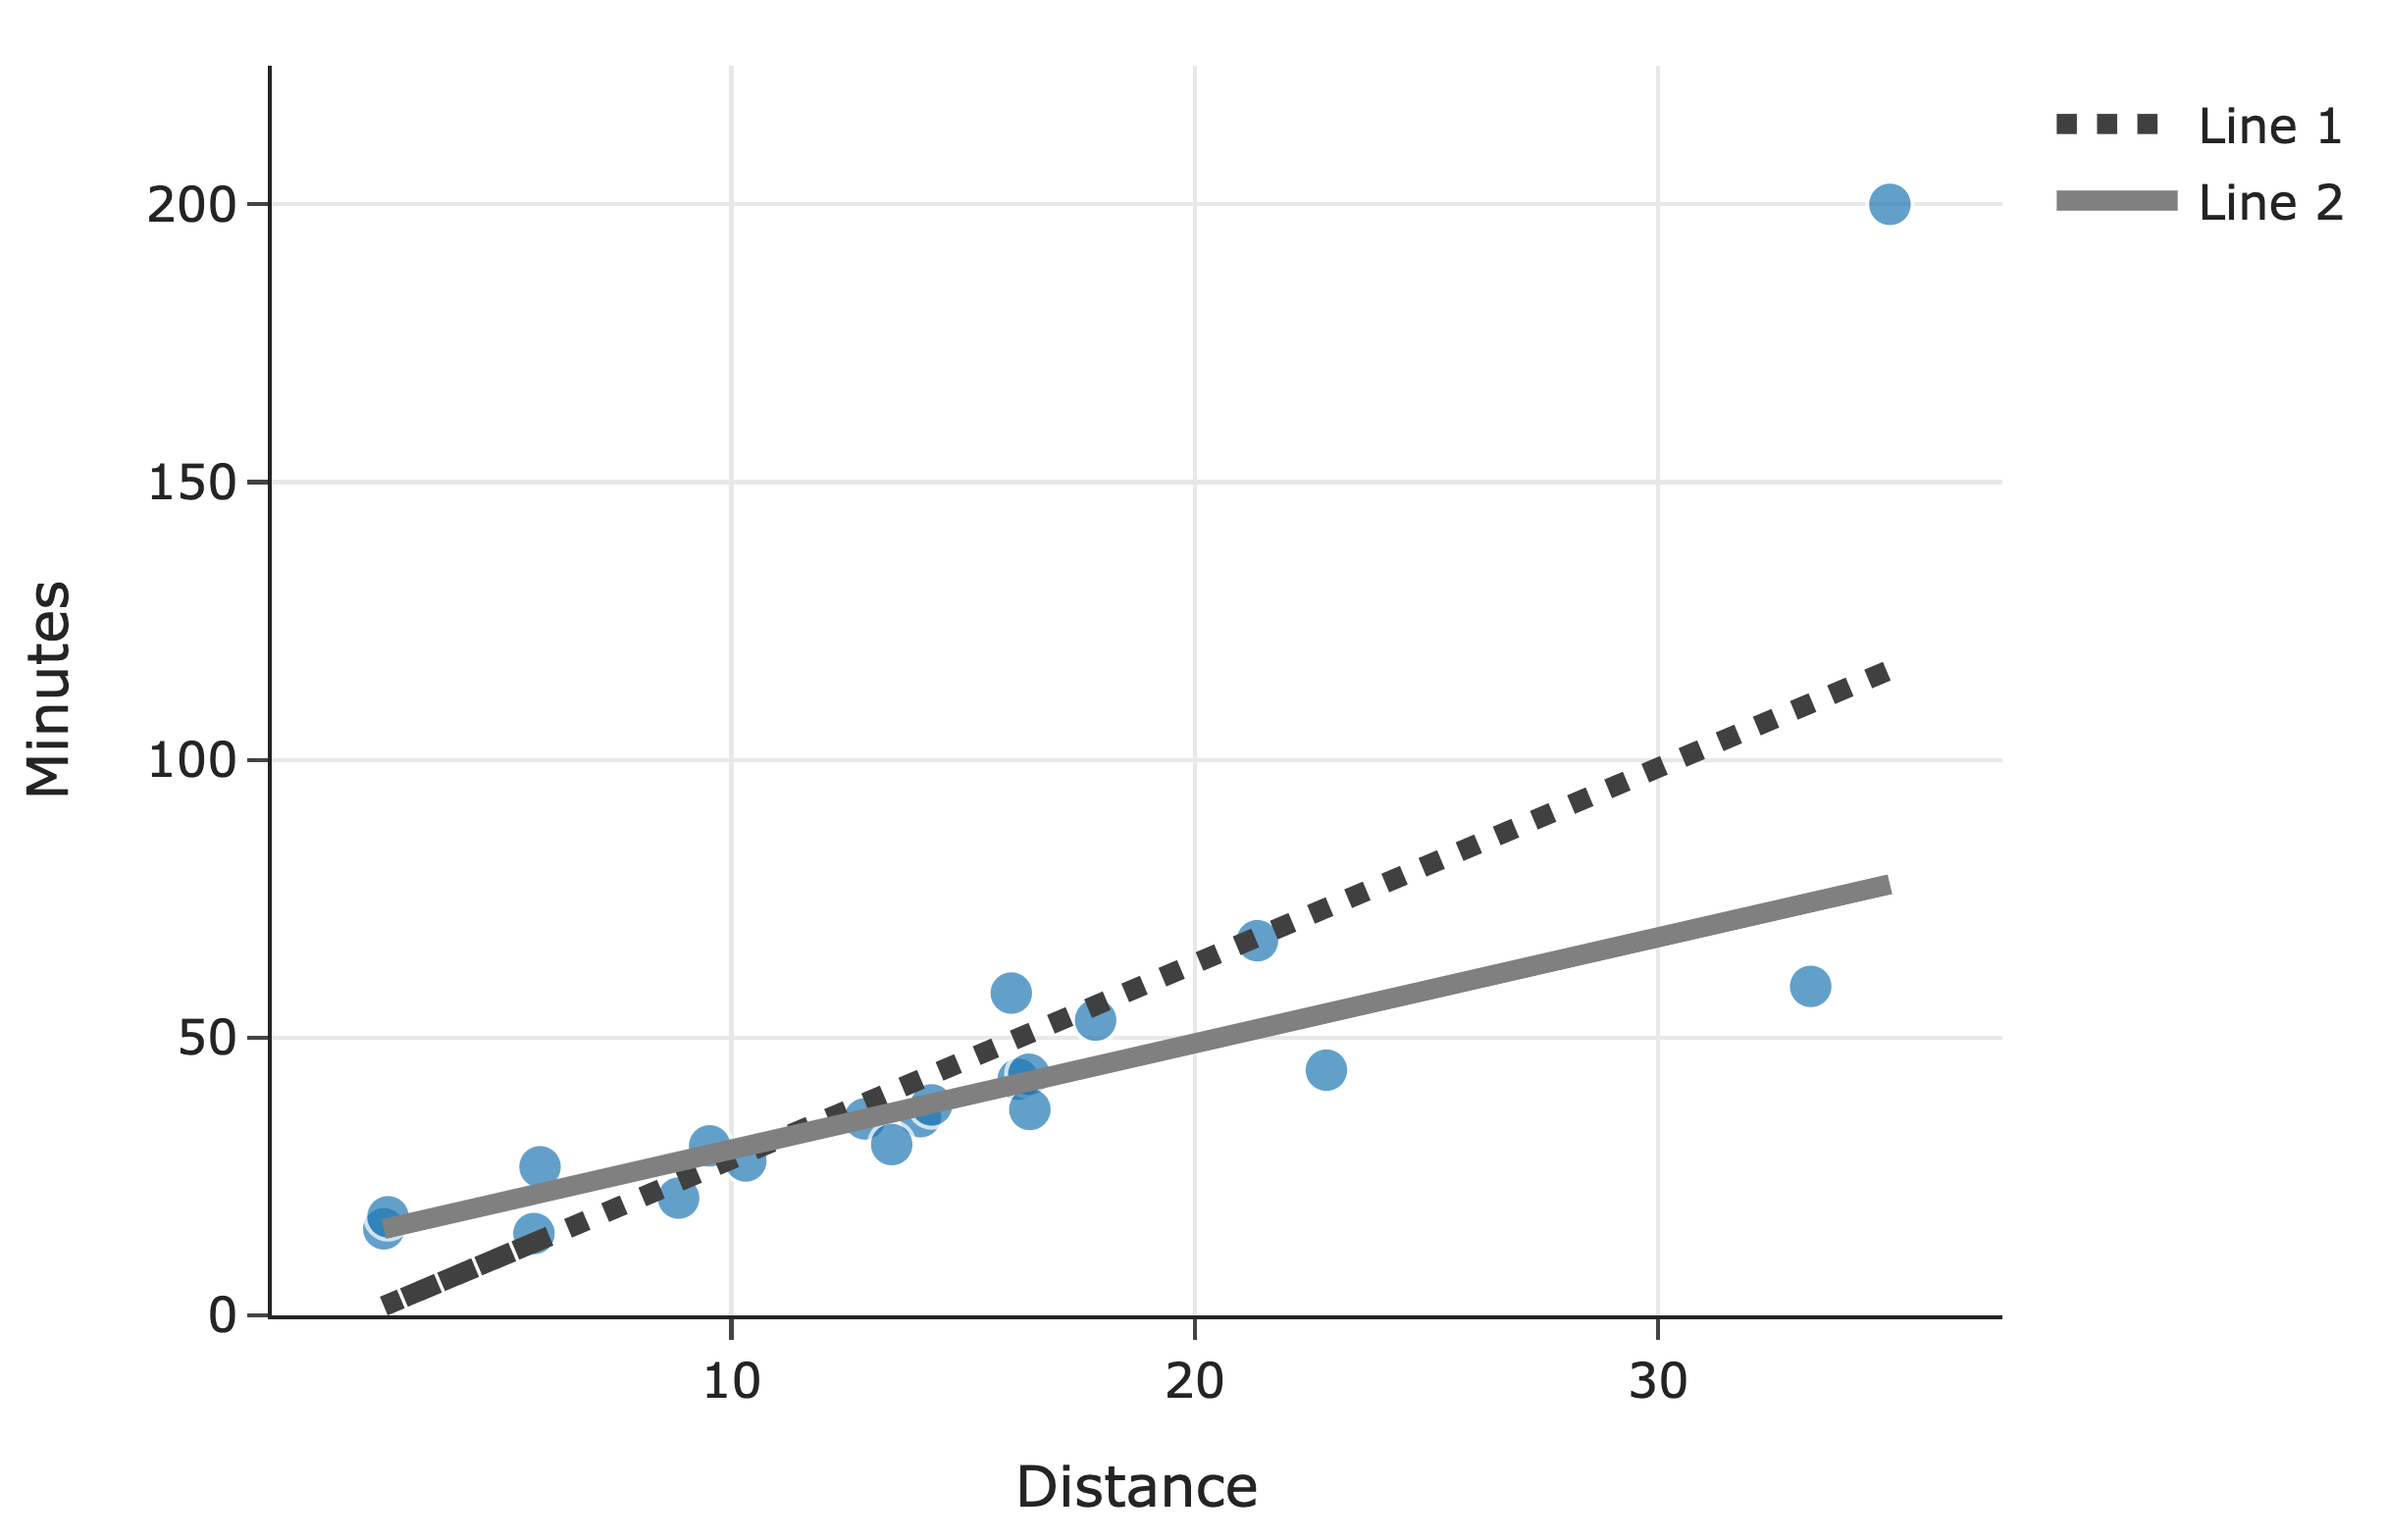
\includegraphics[width=0.5\textwidth]{midterm-images/regression.png}
\end{center}

Which line corresponds to line \textbf{$F$}?
\bubble{Line 1}
\bubble{Line 2}
\end{subprob}

% \begin{subprob}

% Suppose that, in our dataset of $n$ deliveries, there was a \textbf{20 kilometer} delivery that took \textbf{10 minutes}.

% Fill in the \boxed{???}: $$(10 - G(20))^2 \:\:\: \boxed{???} \:\:\: (10 - F(20))^2$$

% \bubble{$\geq$} \bubble{$>$} \bubble{$=$} \bubble{$<$} \bubble{$\leq$} \bubble{Impossible to tell}

% \end{subprob}

% \begin{subprob}

% Suppose that, in our dataset of $n$ deliveries, there was a \textbf{10 kilometer} delivery that took \textbf{40 minutes}.

% Fill in the \boxed{???}: $$(40 - G(10))^2 \:\:\: \boxed{???} \:\:\: (40 - F(10))^2$$

% \bubble{$\geq$} \bubble{$>$} \bubble{$=$} \bubble{$<$} \bubble{$\leq$} \bubble{Impossible to tell}


% \end{subprob}

% \begin{subprob}

% Fill in the blank: $\displaystyle G(\bar{x}) \:\: \rule{0.5cm}{0.15mm} \:\:\: \bar{y}$

% \bubble{$\geq$} \bubble{$>$} \bubble{$=$} \bubble{$<$} \bubble{$\leq$} \bubble{Impossible to tell}

% \end{subprob}

\end{subprobset}

\end{prob}

\newpage

\begin{prob}[(0.5 pts; extra credit)]

In Question 7, assuming that there are 100 unique drivers, what is the true, theoretical probability that \texttt{"WOLVAA01"} wins a free gift card? Show your work, and \boxed{\text{box}} your final answer, which should be a \textbf{fraction}.

Don't spend time on this question if you haven't attempted all other questions, as it is purely for (very little) extra credit.

\begin{responsebox}{3in}
    
\end{responsebox}

\end{prob}

\newpage

Make sure you've written your uniqname in the space provided in the top right corner of every page of this exam.

Congrats on finishing the exam! We hope you enjoy your Spring Break, and wish you the best of luck on any other midterms you may have.

Feel free to draw us a picture about Practical Data Science below :)

% (1 pt) And here's a free point!

\begin{responsebox}{7in}
    
\end{responsebox}

\end{probset}

\end{document}
